% !TEX root = deckblatt3a.tex

\section{Nichtinvertierender Verst\"arker}

\begin{figure}[H]
 \centering
 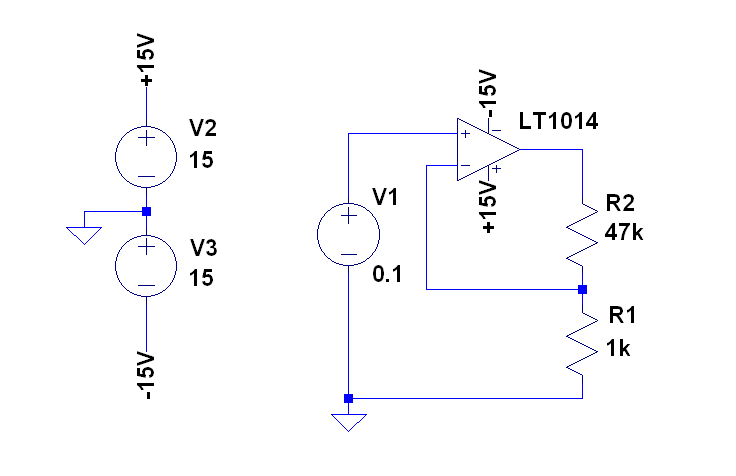
\includegraphics[height=8cm,width=12cm]{Simulationen/OPV}
 \caption{Operationsverstärker beschaltet}
\end{figure}

Die Widerstände wurden im $k\Omega$-Bereich gewählt, um die den Messfehler der Messgeräte möglichst gering zu halten. Die Verstärkung des Operationsverstärker setzt
sich aus dem Verhältniss der beiden Widerstände zusammen, $V_u=1+\frac{47k\Omega}{1k\Omega}=48$, daraus ergeben sich folgende Messwerte.\\

\begin{figure}[H]
 \centering
 \begin{tabular}{c|c}
 $U_e$ 		& $0,1V$ 	\\ \hline
 $U_a$ 		& $4,79V$ 	\\ \hline
 $U_{R1}$ 	& $0,1V$ 	\\ \hline
 $U_{in+}$	& $0,1V$ 	\\ \hline
 $U_{in-}$ 	& $0,99V$ 	\\ \hline
 $I_{R1}$ 	& $0,1mA$ 	\\ \hline
 $I_{R2}$ 	& $0,1mA$ 	\\ \hline
 $I_{in+}$ 	& $0mA$ 	\\ \hline
 $I_{in-}$ 	& $0mA$ 	\\ \hline
 \end{tabular}
 \caption{Simulierte Daten}
\end{figure}

Die Messdaten der Simulation zeigen die zuvor berechnete 48fache Verstärkung der Ausgangsspannung, sowie nahezu keinen Potentialunterschied zwischen den Steuereingängen.
Daher ist auch die Spannung die am Widerstand $R_1$ abgfällt gleich der Eingangsspannung. Die Ströme an den Eingängen des Operationsverstärkers sind gleich $0mA$, da er
sehr hohen Innenwiderstände besitzt. Dadurch fließtauch über beide Widerstände der gleiche Strom. Dies erlaubt es, die Ausgangsspannung über die Spannungsteilerregel zu
berechnen.\\

\begin{align*}
 \frac{U_a}{U_e} &= \frac{R_1 + R_2}{R_1}\\
 U_a &= U_e \left( 1+\frac{R_2}{R_1} \right)\\
\end{align*}

\subsection{Frequenzverhalten}

\begin{figure}[H]
  \centering
  \begin{tikzpicture}
    \begin{axis}[width=15cm, height=10cm, xmin=0, xmax=100e-3, xlabel={t}, ylabel={$U_e$},y tick label style={grid=major}]
      \addplot table[x=time, y=V(n001), mark=none] {csv_files/OPV_Ue_1.csv};
      \addplot table[x=time, y=V(n002), mark=none] {csv_files/OPV_Ua_1.csv};
    \end{axis}
  \end{tikzpicture}
  \caption{symmetrisches Rechtecksignal, $V_{PP}=0.2V, f=100Hz$}
\end{figure}

\begin{figure}[H]
  \centering
  \begin{tikzpicture}
    \begin{axis}[width=15cm, height=10cm, xmin=0, xmax=1e-3, xlabel={t}, ylabel={$U_e$},y tick label style={grid=major}]
      \addplot table[x=time, y=V(n001), mark=none] {csv_files/OPV_Ue_2.csv};
      \addplot table[x=time, y=V(n002), mark=none] {csv_files/OPV_Ua_2.csv};
    \end{axis}
  \end{tikzpicture}
  \caption{symmetrisches Rechtecksignal, $V_{PP}=0.2V, f=10kHz$}
\end{figure}

Der Operationsverstärker besitzt auf Grund seiner Bauweise ein Tiefpassfilter-Verhalten 1.Ordnung. Dies führt dazu, dass die Verstärkung ab einer Grenzfrequenz,
von ca. $1kHz$, mit $20db/DEK$ abnimmt. Bei einer Transitfrequenz von ca. $10MHz$ ist keine Verstärkung mehr vorhanden.\\
Dies kann man gut an den beiden Simulationen erkennen. In der zweiten Simulation kann man erkennen, wie der interne Kondensator bei hohen Frequenzen das Signal
beeinflusst.\\
